% Options for packages loaded elsewhere
\PassOptionsToPackage{unicode}{hyperref}
\PassOptionsToPackage{hyphens}{url}
%
\documentclass[
  english,
  man]{article}
\author{\phantom{0}}
\date{}

\usepackage{amsmath,amssymb}
\usepackage{lmodern}
\usepackage{iftex}
\ifPDFTeX
  \usepackage[T1]{fontenc}
  \usepackage[utf8]{inputenc}
  \usepackage{textcomp} % provide euro and other symbols
\else % if luatex or xetex
  \usepackage{unicode-math}
  \defaultfontfeatures{Scale=MatchLowercase}
  \defaultfontfeatures[\rmfamily]{Ligatures=TeX,Scale=1}
\fi
% Use upquote if available, for straight quotes in verbatim environments
\IfFileExists{upquote.sty}{\usepackage{upquote}}{}
\IfFileExists{microtype.sty}{% use microtype if available
  \usepackage[]{microtype}
  \UseMicrotypeSet[protrusion]{basicmath} % disable protrusion for tt fonts
}{}
\makeatletter
\@ifundefined{KOMAClassName}{% if non-KOMA class
  \IfFileExists{parskip.sty}{%
    \usepackage{parskip}
  }{% else
    \setlength{\parindent}{0pt}
    \setlength{\parskip}{6pt plus 2pt minus 1pt}}
}{% if KOMA class
  \KOMAoptions{parskip=half}}
\makeatother
\usepackage{xcolor}
\IfFileExists{xurl.sty}{\usepackage{xurl}}{} % add URL line breaks if available
\IfFileExists{bookmark.sty}{\usepackage{bookmark}}{\usepackage{hyperref}}
\hypersetup{
  pdflang={en-EN},
  hidelinks,
  pdfcreator={LaTeX via pandoc}}
\urlstyle{same} % disable monospaced font for URLs
\usepackage{longtable,booktabs,array}
\usepackage{calc} % for calculating minipage widths
% Correct order of tables after \paragraph or \subparagraph
\usepackage{etoolbox}
\makeatletter
\patchcmd\longtable{\par}{\if@noskipsec\mbox{}\fi\par}{}{}
\makeatother
% Allow footnotes in longtable head/foot
\IfFileExists{footnotehyper.sty}{\usepackage{footnotehyper}}{\usepackage{footnote}}
\makesavenoteenv{longtable}
\usepackage{graphicx}
\makeatletter
\def\maxwidth{\ifdim\Gin@nat@width>\linewidth\linewidth\else\Gin@nat@width\fi}
\def\maxheight{\ifdim\Gin@nat@height>\textheight\textheight\else\Gin@nat@height\fi}
\makeatother
% Scale images if necessary, so that they will not overflow the page
% margins by default, and it is still possible to overwrite the defaults
% using explicit options in \includegraphics[width, height, ...]{}
\setkeys{Gin}{width=\maxwidth,height=\maxheight,keepaspectratio}
% Set default figure placement to htbp
\makeatletter
\def\fps@figure{htbp}
\makeatother
\setlength{\emergencystretch}{3em} % prevent overfull lines
\providecommand{\tightlist}{%
  \setlength{\itemsep}{0pt}\setlength{\parskip}{0pt}}
\setcounter{secnumdepth}{-\maxdimen} % remove section numbering
% Make \paragraph and \subparagraph free-standing
\ifx\paragraph\undefined\else
  \let\oldparagraph\paragraph
  \renewcommand{\paragraph}[1]{\oldparagraph{#1}\mbox{}}
\fi
\ifx\subparagraph\undefined\else
  \let\oldsubparagraph\subparagraph
  \renewcommand{\subparagraph}[1]{\oldsubparagraph{#1}\mbox{}}
\fi
\newlength{\cslhangindent}
\setlength{\cslhangindent}{1.5em}
\newlength{\csllabelwidth}
\setlength{\csllabelwidth}{3em}
\newlength{\cslentryspacingunit} % times entry-spacing
\setlength{\cslentryspacingunit}{\parskip}
\newenvironment{CSLReferences}[2] % #1 hanging-ident, #2 entry spacing
 {% don't indent paragraphs
  \setlength{\parindent}{0pt}
  % turn on hanging indent if param 1 is 1
  \ifodd #1
  \let\oldpar\par
  \def\par{\hangindent=\cslhangindent\oldpar}
  \fi
  % set entry spacing
  \setlength{\parskip}{#2\cslentryspacingunit}
 }%
 {}
\usepackage{calc}
\newcommand{\CSLBlock}[1]{#1\hfill\break}
\newcommand{\CSLLeftMargin}[1]{\parbox[t]{\csllabelwidth}{#1}}
\newcommand{\CSLRightInline}[1]{\parbox[t]{\linewidth - \csllabelwidth}{#1}\break}
\newcommand{\CSLIndent}[1]{\hspace{\cslhangindent}#1}
% Manuscript styling
\usepackage{upgreek}
\captionsetup{font=singlespacing,justification=justified}

% Table formatting
\usepackage{longtable}
\usepackage{lscape}
% \usepackage[counterclockwise]{rotating}   % Landscape page setup for large tables
\usepackage{multirow}		% Table styling
\usepackage{tabularx}		% Control Column width
\usepackage[flushleft]{threeparttable}	% Allows for three part tables with a specified notes section
\usepackage{threeparttablex}            % Lets threeparttable work with longtable

% Create new environments so endfloat can handle them
% \newenvironment{ltable}
%   {\begin{landscape}\begin{center}\begin{threeparttable}}
%   {\end{threeparttable}\end{center}\end{landscape}}
\newenvironment{lltable}{\begin{landscape}\begin{center}\begin{ThreePartTable}}{\end{ThreePartTable}\end{center}\end{landscape}}

% Enables adjusting longtable caption width to table width
% Solution found at http://golatex.de/longtable-mit-caption-so-breit-wie-die-tabelle-t15767.html
\makeatletter
\newcommand\LastLTentrywidth{1em}
\newlength\longtablewidth
\setlength{\longtablewidth}{1in}
\newcommand{\getlongtablewidth}{\begingroup \ifcsname LT@\roman{LT@tables}\endcsname \global\longtablewidth=0pt \renewcommand{\LT@entry}[2]{\global\advance\longtablewidth by ##2\relax\gdef\LastLTentrywidth{##2}}\@nameuse{LT@\roman{LT@tables}} \fi \endgroup}

% \setlength{\parindent}{0.5in}
% \setlength{\parskip}{0pt plus 0pt minus 0pt}

% Overwrite redefinition of paragraph and subparagraph by the default LaTeX template
% See https://github.com/crsh/papaja/issues/292
\makeatletter
\renewcommand{\paragraph}{\@startsection{paragraph}{4}{\parindent}%
  {0\baselineskip \@plus 0.2ex \@minus 0.2ex}%
  {-1em}%
  {\normalfont\normalsize\bfseries\itshape\typesectitle}}

\renewcommand{\subparagraph}[1]{\@startsection{subparagraph}{5}{1em}%
  {0\baselineskip \@plus 0.2ex \@minus 0.2ex}%
  {-\z@\relax}%
  {\normalfont\normalsize\itshape\hspace{\parindent}{#1}\textit{\addperi}}{\relax}}
\makeatother

% \usepackage{etoolbox}
\makeatletter
\patchcmd{\HyOrg@maketitle}
  {\section{\normalfont\normalsize\abstractname}}
  {\section*{\normalfont\normalsize\abstractname}}
  {}{\typeout{Failed to patch abstract.}}
\patchcmd{\HyOrg@maketitle}
  {\section{\protect\normalfont{\@title}}}
  {\section*{\protect\normalfont{\@title}}}
  {}{\typeout{Failed to patch title.}}
\makeatother
\keywords{Retroactive Interference, Memory Consolidation\newline\indent Word count: X}
\DeclareDelayedFloatFlavor{ThreePartTable}{table}
\DeclareDelayedFloatFlavor{lltable}{table}
\DeclareDelayedFloatFlavor*{longtable}{table}
\makeatletter
\renewcommand{\efloat@iwrite}[1]{\immediate\expandafter\protected@write\csname efloat@post#1\endcsname{}}
\makeatother
\usepackage{lineno}

\linenumbers
\usepackage{csquotes}
\ifXeTeX
  % Load polyglossia as late as possible: uses bidi with RTL langages (e.g. Hebrew, Arabic)
  \usepackage{polyglossia}
  \setmainlanguage[]{english}
\else
  \usepackage[main=english]{babel}
% get rid of language-specific shorthands (see #6817):
\let\LanguageShortHands\languageshorthands
\def\languageshorthands#1{}
\fi
\ifLuaTeX
  \usepackage{selnolig}  % disable illegal ligatures
\fi


\shorttitle{SHORT TITLE}

\affiliation{\phantom{0}}

\begin{document}

\begin{longtable}[]{@{}
  >{\raggedright\arraybackslash}p{(\columnwidth - 0\tabcolsep) * \real{0.06}}@{}}
\toprule
\endhead
title : ``Replication of Darby and Sloutsky (2015) analysis''
shorttitle : ``Semester project'' \\
author:
- name : ``Scarlett Reynoso Moreno''
affiliation : ``1''
corresponding : yes \# Define only one corresponding author
address : ``365 5th Ave, New York, NY 10016''
email : ``\href{mailto:leavesofnyc@gmail.com}{\nolinkurl{leavesofnyc@gmail.com}}'' \\
affiliation:
- id : ``1''
institution : ``CUNY BA for Unique and Interdisciplinary Studies'' \\
authornote: \textbar{}
Fill \\
abstract: \textbar{} \\
keywords : ``Retroactive Interference, Memory Consolidation''
wordcount : ``X'' \\
bibliography : {[}``r-references.bib,''``references.bib''{]} \\
floatsintext : no
figurelist : no
tablelist : no
footnotelist : no
linenumbers : yes
mask : no
draft : no \\
documentclass : ``apa6''
classoption : ``man''
output : papaja::apa6\_pdf \\
\bottomrule
\end{longtable}

\hypertarget{introduction}{%
\subsection{Introduction}\label{introduction}}

Recent research has suggested that children experience catastrophic interference of memory at a much higher rate than adults. This means that when new learning takes place, old learning can fade in children. This effect is rarely seen in adults. Darby and Sloutsky (2015) designed an experiment to test the affect of delays between learning and testing to find out if time assists in preventing retroactive interference.

Importing data

\begin{verbatim}
## Warning: package 'dplyr' was built under R version 4.0.5
\end{verbatim}

\begin{verbatim}
## Warning: package 'ggplot2' was built under R version 4.0.5
\end{verbatim}

\begin{verbatim}
## [1] "Experiment_1_No_Delay"            "Experiment_1_Delay_After_Phase_2"
## [3] "Experiment_2_Delay_After_Phase_1"
\end{verbatim}

\begin{verbatim}
## # A tibble: 30 x 4
## # Groups:   Block, Phase [15]
##    Block Phase Pair_type     Avg
##    <dbl> <dbl> <chr>       <dbl>
##  1     1     1 overlapping  0.6 
##  2     1     1 unique       0.56
##  3     1     2 overlapping  0.48
##  4     1     2 unique       0.7 
##  5     1     3 overlapping  0.64
##  6     1     3 unique       0.88
##  7     2     1 overlapping  0.91
##  8     2     1 unique       0.88
##  9     2     2 overlapping  0.78
## 10     2     2 unique       0.93
## # ... with 20 more rows
\end{verbatim}

\begin{table}[tbp]

\begin{center}
\begin{threeparttable}

\caption{\label{tab:unnamed-chunk-1}Average Accuracy Means}

\begin{tabular}{llll}
\toprule
Block & \multicolumn{1}{c}{Phase} & \multicolumn{1}{c}{Pair\_type} & \multicolumn{1}{c}{Avg}\\
\midrule
1.00 & 1.00 & overlapping & 0.60\\
1.00 & 1.00 & unique & 0.56\\
1.00 & 2.00 & overlapping & 0.48\\
1.00 & 2.00 & unique & 0.70\\
1.00 & 3.00 & overlapping & 0.64\\
1.00 & 3.00 & unique & 0.88\\
2.00 & 1.00 & overlapping & 0.91\\
2.00 & 1.00 & unique & 0.88\\
2.00 & 2.00 & overlapping & 0.78\\
2.00 & 2.00 & unique & 0.93\\
2.00 & 3.00 & overlapping & 0.85\\
2.00 & 3.00 & unique & 0.93\\
3.00 & 1.00 & overlapping & 0.91\\
3.00 & 1.00 & unique & 0.88\\
3.00 & 2.00 & overlapping & 0.91\\
3.00 & 2.00 & unique & 0.93\\
3.00 & 3.00 & overlapping & 0.89\\
3.00 & 3.00 & unique & 0.96\\
4.00 & 1.00 & overlapping & 0.92\\
4.00 & 1.00 & unique & 0.93\\
4.00 & 2.00 & overlapping & 0.88\\
4.00 & 2.00 & unique & 0.97\\
4.00 & 3.00 & overlapping & 0.93\\
4.00 & 3.00 & unique & 0.92\\
5.00 & 1.00 & overlapping & 0.93\\
5.00 & 1.00 & unique & 0.92\\
5.00 & 2.00 & overlapping & 0.91\\
5.00 & 2.00 & unique & 0.97\\
5.00 & 3.00 & overlapping & 0.95\\
5.00 & 3.00 & unique & 0.94\\
\bottomrule
\end{tabular}

\end{threeparttable}
\end{center}

\end{table}

\hypertarget{methods}{%
\section{Methods}\label{methods}}

\hypertarget{participants}{%
\subsection{Participants}\label{participants}}

The participants of experiment 1, no delay condition were forty pre-school aged children ranging in ages between 4.6 and 5.8 with a gender breakdown of 22 girls to 18 boys @ darby2015delays.

\hypertarget{material}{%
\subsection{Material}\label{material}}

The experimental questions related to this replication study can be found in (\textbf{darby2015delays?}).

\hypertarget{procedure}{%
\subsection{Procedure}\label{procedure}}

In experiment 1, no delay condition, participants took part in three phases deciding which two commonplace objects were associated with the cartoon character Mickey Mouse or Pooh Bear. The trials that composed the three phases were either associated with an ``overlapping'' condition or a ``unique'' condition. If participants were a part of ``overlapping'' trials, then one of the two commonplace objects associated to a cartoon character in phase 1 would be recombined with a different second object in phase two. Then in phase 3 participants were tested to see if they still remembered the two objects associated to a cartoon character in phase 1. If participants were a part of ``unique'' trials, then the two objects associated with a cartoon character in phase 1 were not present in phase 2.

Variables : delay and no delay w/ overlapping and unique levels

\begin{verbatim}
## # A tibble: 25 x 2
##    Subject AvgAccuracy
##      <dbl>       <dbl>
##  1    3049       0.95 
##  2    3052       0.75 
##  3    3053       0.817
##  4    3056       0.933
##  5    3066       0.833
##  6    3068       0.85 
##  7    3069       0.85 
##  8    3070       0.85 
##  9    3073       0.8  
## 10    3082       0.883
## # ... with 15 more rows
\end{verbatim}

\begin{verbatim}
## # A tibble: 25 x 2
##    Subject AvgAccuracy
##      <dbl>       <dbl>
##  1    3049       0.933
##  2    3052       0.833
##  3    3053       0.9  
##  4    3056       0.917
##  5    3066       0.917
##  6    3068       0.917
##  7    3069       0.817
##  8    3070       0.917
##  9    3073       0.917
## 10    3082       0.983
## # ... with 15 more rows
\end{verbatim}

\begin{verbatim}
## 
##  Paired t-test
## 
## data:  Experiment_1_No_Delay_overlapping$AvgAccuracy and Experiment_1_No_Delay_unique$AvgAccuracy
## t = -4.4053, df = 24, p-value = 0.0001885
## alternative hypothesis: true difference in means is not equal to 0
## 95 percent confidence interval:
##  -0.07929933 -0.02870067
## sample estimates:
## mean of the differences 
##                  -0.054
\end{verbatim}

\hypertarget{power-curve---simulation-based-power-analysis}{%
\subsubsection{Power curve - Simulation-based power analysis}\label{power-curve---simulation-based-power-analysis}}

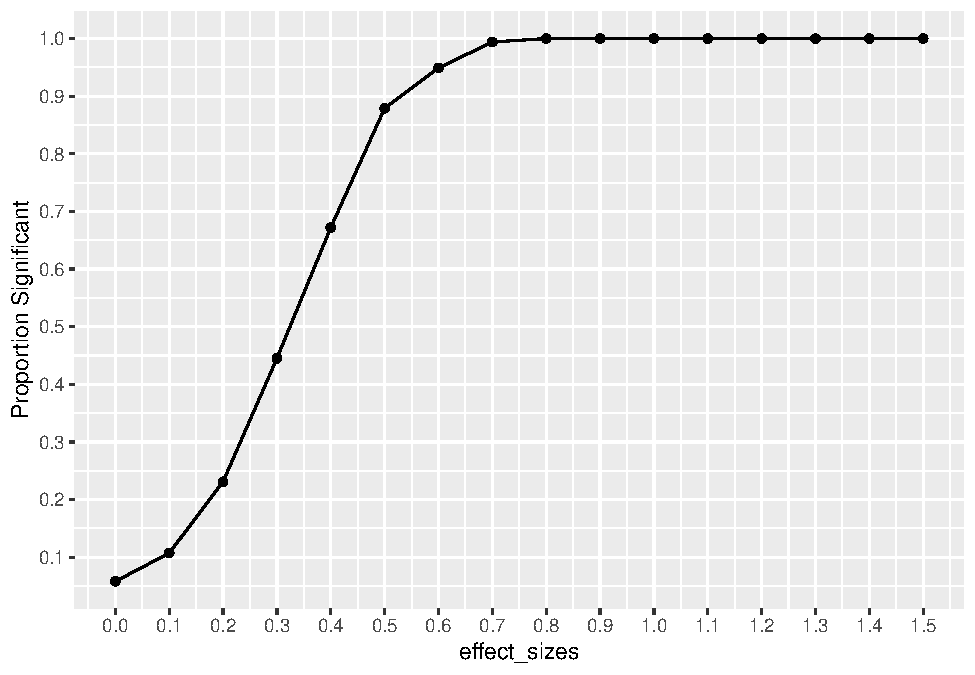
\includegraphics{Reproduced-analysis_stats_I_files/figure-latex/unnamed-chunk-3-1.pdf}

\hypertarget{results}{%
\subsubsection{Results}\label{results}}

No-delay condition, Darby and Sloutsky (2015) found that accuracy significantly decreased in overlapping pairs, t(24) = 6.82. p \textless.001, Cohen's d = 1.39. In unique pairs there was not significance, p = .46.

\newpage

\hypertarget{references}{%
\section{References}\label{references}}

\begingroup
\setlength{\parindent}{-0.5in}
\setlength{\leftskip}{0.5in}

\hypertarget{refs}{}
\begin{CSLReferences}{0}{0}
\end{CSLReferences}

\endgroup


\end{document}
